\chapter{측정, 밀도 행렬, 엔트로피}

이중 슬릿 실험에는 유용한 최소한의 형태로 측정 문제가 담겨 있다. 두 대안이 결맞음을 유지하면 진폭이 간섭한다. 다른 계가 어떤 대안을 택했는지 기록하면 입자와 기록 장치가 얽히고 간섭 양상도 달라진다. 부분 추적, 밀도 행렬, 엔트로피를 도입하기에 앞서 이 메커니즘을 정확히 살펴보자---얽힘을 정량화하는 데 필요한 언어다.

\section{이중 슬릿 실험 다시 구성하기}

위치 \(0\)에 있는 광원, 두 개의 구멍 \(A\)와 \(B\), 그리고 도착 가능한 위치를 정규직교 상태 \(\{|m\rangle\}\)로 나타낸 스크린이 있는 이산 모형을 생각하자. 입자는 전자, 광자 또는 다른 어떤 양자 물체여도 된다. 여기서는 이를 전자라고 부르고, 위치만 논의하도록 전자의 스핀은 무시한다. 장벽의 나머지 부분은 막혀 있다. \(A\) 또는 \(B\) 이외의 위치에 도달한 전자는 반사된다.

핵심 원리는 선형성이다. 두 상태가 다음과 같이 시간에 따라 변한다면
\begin{equation}
|A\rangle\longrightarrow |A'\rangle,
\qquad
|B\rangle\longrightarrow |B'\rangle,
\end{equation}
모든 중첩도 같은 계수를 유지하며 다음과 같이 변한다.
\begin{equation}
\alpha|A\rangle+\beta|B\rangle
\longrightarrow
\alpha|A'\rangle+\beta|B'\rangle.
\end{equation}

대칭적인 배열에서는 광원이 두 구멍에 같은 진폭으로 입사시킨다. 칠판에서처럼 공통 정규화 인자를 생략하면,
\begin{equation}
|0\rangle\longrightarrow |A\rangle+|B\rangle.
\end{equation}
정규화된 상태는 \((|A\rangle+|B\rangle)/\sqrt{2}\)이다. 생략한 인자는 간섭 논증에 아무런 역할도 하지 않는다.

이제 각 경로를 따로 살펴보자. 구멍에서 스크린까지의 전파는 다음과 같은 형태다.
\begin{align}
|A\rangle &\longrightarrow \sum_m \psi_m|m\rangle, \\
|B\rangle &\longrightarrow \sum_m \phi_m|m\rangle.
\end{align}
복소수 \(\psi_m\)는 \(A\)에서 출발해 스크린 위치 \(m\)에 도달할 진폭이고, \(\phi_m\)는 \(B\)에서 출발했을 때의 해당 진폭이다.

\begin{figure}[htbp]
\centering
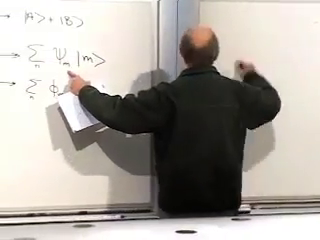
\includegraphics[width=0.68\textwidth]{lecture_07_figure_02.png}
\caption{스크린 기저에서 전개한 \(A\) 경로와 \(B\) 경로의 각각의 상태.}
\lectureframe{00:05:39}
\end{figure}

\(B\)을 막으면 위치 \(m\)에서의 확률은
\begin{equation}
P_A(m)=|\psi_m|^2.
\end{equation}
\(A\)를 막으면,
\begin{equation}
P_B(m)=|\phi_m|^2.
\end{equation}
고전 확률이라면 두 구멍이 모두 열려 있을 때 이 두 결과를 더해야 한다고 볼 것이다. 그러나 양자역학에서는 먼저 진폭을 더한다.
\begin{equation}
|A\rangle+|B\rangle
\longrightarrow
\sum_m(\psi_m+\phi_m)|m\rangle.
\end{equation}
스크린의 특정 위치에서,
\begin{align}
P(m)
&=|\psi_m+\phi_m|^2 \\
&=|\psi_m|^2+|\phi_m|^2
  +\psi_m^*\phi_m+\phi_m^*\psi_m.
\end{align}

\begin{figure}[htbp]
\centering
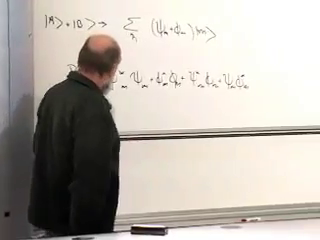
\includegraphics[width=0.70\textwidth]{lecture_07_figure_03.png}
\caption{스크린에서의 네 항 확률. 마지막 두 항은 간섭항이다.}
\lectureframe{00:09:21}
\end{figure}

대칭점에서는 \(\psi_m=\phi_m\)가 성립하여 두 대안이 서로 보강한다. 두 대안의 위상 차이가 \(\pi\)인 점, 즉 \(\psi_m=-\phi_m\)인 점에서는 확률이 사라진다. 어느 한 경로만으로도 그 점에 도달할 수 있지만, 두 경로를 모두 열면 전자가 그곳에 도달하지 못할 수 있다. 이제 다음 질문을 피할 수 없다. 어느 구멍을 통과했는지 기록하는 무언가가 생기면 무엇이 달라지는가?

\section{검출기와 얽히다}

상태 \(|u\rangle\)와 \(|d\rangle\)를 갖는 보조 2상태 계를 도입하자. 이 모형에서 이 계는 전자의 스핀이 아니라 최소한의 외부 장치다. 처음에 검출기는 작동하지 않은 상태다.
\begin{equation}
|0,d\rangle.
\end{equation}
\(A\)을 통과하면 검출기 상태가 뒤집히고, \(B\)을 통과하면 그대로 유지되도록 상호작용을 설정하자.
\begin{equation}
|0,d\rangle
\longrightarrow
|A,u\rangle+|B,d\rangle.
\end{equation}
전자가 구멍을 지난 뒤에는 보조 스핀과 더 이상 상호작용하지 않는다. 따라서 두 갈래는 다음과 같이 전파되고,
\begin{align}
|A,u\rangle &\longrightarrow \sum_m\psi_m|m,u\rangle, \\
|B,d\rangle &\longrightarrow \sum_m\phi_m|m,d\rangle,
\end{align}
최종 상태는 다음과 같다.
\begin{equation}
|\Psi\rangle
=\sum_m\left(\psi_m|m,u\rangle+\phi_m|m,d\rangle\right).
\end{equation}
이제 경로와 검출기의 기록이 얽혀 있다. 검출기를 읽으면 어느 구멍을 통과했는지 알 수 있다.

\begin{classroomqa}
\lecturetimestamp{00:13:24}
\audiencequestion{스핀이 뒤집히면 파동 묶음은 이미 붕괴한 것인가?}
\lecturerresponse{전자만 놓고 보면 경로 대안들이 더는 간섭하지 않는다는 뜻으로 붕괴라는 표현을 쓸 수 있다. 그러나 전자--검출기 전체 계에서는 어느 갈래도 버려지지 않았다. 상태는 여전히 \(|A,u\rangle+|B,d\rangle\)이다. 장치까지 포함하면 \emph{전자가 붕괴했다}는 표현은 계--장치의 얽힘이 형성되었다는 정확한 표현으로 대체된다.}
\end{classroomqa}

보조 스핀은 편리한 지시자일 뿐이다. 작동한 장치와 작동하지 않은 장치, 방출된 광자와 방출되지 않은 광자, 또는 서로 구별되는 다른 어떤 두 기록 상태도 같은 역할을 할 수 있다.

\begin{classroomqa}
\lecturetimestamp{00:15:17}
\audiencequestion{금속판을 통과하면 언제나 경로 기록이 남는가?}
\lecturerresponse{반드시 그렇지는 않다. 중요한 것은 상호작용으로 판이 구별 가능한 최종 상태에 놓이는가이다. 판에 여기 에너지 간격이 있고 전자의 에너지가 판을 여기시키기에 충분하지 않다면, 지속되는 내부 흔적이 남지 않을 수도 있다. 상호작용만으로는 충분하지 않다. 두 대안이 구별 가능한 기록과 상관관계를 이루어야 한다.}
\end{classroomqa}

\begin{classroomqa}
\lecturetimestamp{00:16:29}
\audiencequestion{판의 반동으로 전자가 위쪽과 아래쪽 중 어느 구멍을 통과했는지 알 수 있는가?}
\lecturerresponse{서로 반대 방향의 운동량 충격이 판을 충분히 구별 가능한 상태로 만들 때만 가능하다. 위치가 잘 국소화된 판은 이미 폭이 넓은 운동량 파동함수를 갖는다. 위아래로 조금씩 이동한 상태는 거의 완전히 겹칠 수 있으므로, 반동 상태들은 직교하지 않으며 경로를 확실하게 알려 주지 못한다. 여기서 불확정성 원리가 간섭을 보호한다.}
\end{classroomqa}

부분적인 기록도 가능하다. 검출기가 아주 약하게 밀려나면 두 최종 기록 상태가 직교하지 않을 수 있다. 이 경우 간섭은 사라지는 대신 약해진다. 형식적으로 계산하기 위해 우선 완전 측정이라는 극한적인 경우를 생각하자.
\begin{equation}
\langle u|d\rangle=0.
\end{equation}

\section{사영 연산자로 계산하기}

이제 검출기 결과는 묻지 않고 전자가 스크린의 특정 위치 \(m\)에 도달할 확률을 계산하자. 결합 힐베르트 공간에서 \emph{전자 위치가 \(m\)}이라는 성질은 다음 두 상태가 생성하는 2차원 부분공간에 해당한다.
\begin{equation}
|m,u\rangle,\qquad |m,d\rangle.
\end{equation}
이에 대응하는 사영 연산자는
\begin{equation}
\Pi_m
=|m,u\rangle\langle m,u|
 +|m,d\rangle\langle m,d|.
\end{equation}

\begin{figure}[htbp]
\centering
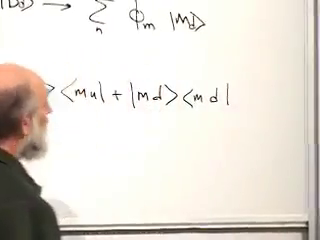
\includegraphics[width=0.66\textwidth]{lecture_07_figure_04.png}
\caption{두 직교 검출 기록에 대해 합한, 스크린의 특정 위치로의 사영 연산자.}
\lectureframe{00:22:04}
\end{figure}

확률 공리에 따르면
\begin{equation}
P(m)=\langle\Psi|\Pi_m|\Psi\rangle.
\end{equation}
합을 풀어 쓰면,
\begin{align}
P(m)
&=
\sum_{n,n'}
\left(\psi_n^*\langle n,u|+\phi_n^*\langle n,d|\right)
\notag\\
&\quad\times\Pi_m
\notag\\
&\quad\times
\left(\psi_{n'}|n',u\rangle+\phi_{n'}|n',d\rangle\right).
\end{align}
위치에 대한 내적은 \(n=m=n'\)을 요구한다. 이어서 검출기 내적에 따라 어떤 항이 남는지가 결정된다.
\begin{align}
\langle u|u\rangle&=1,
&
\langle d|d\rangle&=1,
&
\langle u|d\rangle&=\langle d|u\rangle=0.
\end{align}
따라서,
\begin{equation}
P(m)=|\psi_m|^2+|\phi_m|^2.
\end{equation}

교차항은 임의로 없앤 것이 아니다. 확장된 상태 공간에서 두 경로 진폭이 서로 직교하는 벡터와 곱해지기 때문에 사라진다. 간섭하려면 대안들이 스크린의 종착점에서만 일치해서는 안 된다. 기록을 담고 있는 모든 자유도에서도 일치해야 한다.

\section{무엇을 측정이라고 하는가?}

이 간결한 스핀 모형은 일반적인 규칙을 보여 준다. 계의 대안들과 장치의 구별 가능한 상태들 사이에 상관관계를 형성하는 상호작용이 일어날 때 측정이 성립한다. 다음 사례들로 이 규칙을 살펴보자.

\begin{classroomqa}
\lecturetimestamp{00:26:53}
\audiencequestion{스핀을 대칭적으로 배치하고 어느 구멍을 통과하든 뒤집히게 하면 어떻게 되는가?}
\lecturerresponse{그러면 두 갈래 모두 같은 기록 \(|A,u\rangle+|B,u\rangle=(|A\rangle+|B\rangle)\otimes|u\rangle\)을 갖는다. 검출기 상태는 인수분해되어 경로 정보를 알려 주지 않으므로 간섭 무늬는 그대로 남는다.}
\end{classroomqa}

\begin{figure}[htbp]
\centering
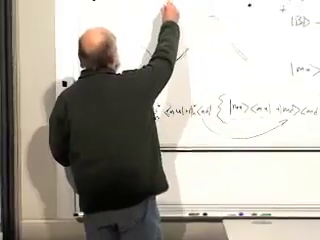
\includegraphics[width=0.68\textwidth]{lecture_07_figure_05.png}
\caption{대칭 위치에 둔 검출기가 두 경로에 똑같이 반응하도록 한 칠판의 변형 사례.}
\lectureframe{00:27:14}
\end{figure}

\begin{figure}[htbp]
\centering
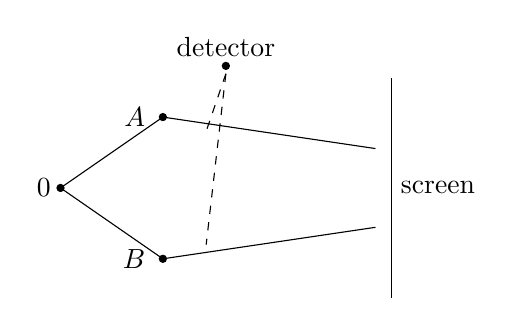
\begin{tikzpicture}[scale=1.0]
\fill (-2,0) circle (1.5pt);
\node[left] at (-2,0) {$0$};
\fill (-0.7,0.9) circle (1.5pt);
\node[left] at (-0.8,0.9) {$A$};
\fill (-0.7,-0.9) circle (1.5pt);
\node[left] at (-0.8,-0.9) {$B$};
\draw (-2,0) -- (-0.7,0.9);
\draw (-2,0) -- (-0.7,-0.9);
\draw (-0.7,0.9) -- (2.0,0.5);
\draw (-0.7,-0.9) -- (2.0,-0.5);
\draw (2.2,-1.4) -- (2.2,1.4);
\node[right] at (2.2,0) {screen};
\fill (0.1,1.55) circle (1.5pt);
\node[above] at (0.1,1.55) {detector};
\draw[dashed] (0.1,1.45) -- (-0.15,0.72);
\draw[dashed] (0.1,1.45) -- (-0.15,-0.72);
\end{tikzpicture}
\caption{대칭적인 검출기 배치를 깔끔하게 재구성한 그림. 두 경로에서 검출기 상태는 동일하다.}
\end{figure}

\begin{classroomqa}
\lecturetimestamp{00:27:55}
\audiencequestion{간섭이 사라지려면 누군가 실제로 보조 스핀을 읽어야 하는가?}
\lecturerresponse{아니다. 전자는 이미 경로와 스핀 사이에 상관관계를 형성했다. 검출기를 초기화하고 전자를 한 번에 하나씩 보내면서 스크린에 도달한 위치 분포만 살펴볼 수 있다. 아무도 스핀을 읽지 않더라도 간섭 무늬는 사라진다. 중요한 것은 기록의 존재이지, 사람이 그 기록을 인식하는지가 아니다.}
\end{classroomqa}

\begin{classroomqa}
\lecturetimestamp{00:29:36}
\audiencequestion{충분히 가벼운 반동 판이라면 간섭을 없앨 수 있는가?}
\lecturerresponse{반동으로 두 경로에서 판이 직교하는 운동량 상태에 놓인다면 그렇다. 이동한 파동 묶음들이 여전히 겹친다면 간섭은 부분적으로만 사라진다. 기준은 질량 자체가 아니라 판의 최종 상태들이 구별 가능한가이다.}
\end{classroomqa}

복사도 불완전한 기록 장치가 될 수 있다. 가속된 하전 입자는 광자를 방출할 수 있다. \(A\) 부근에서 방출된 복사는 \(B\) 부근에서 방출된 복사와 같은 상태가 아닐 수 있으므로, 전자기장은 경로 정보를 보유할 수 있다. 천천히 편향된 전자의 경우 방출 확률은 작을 수 있다. 강의에서는 대략 백 번 중 한 번 일어나는 예시적 추산을 든다. 더 큰 가속은 복사와 그에 따른 대비 감소의 가능성을 높인다. 핵심은 정성적인 점이다. 관측되지 않은 광자도 결맞음을 가져갈 수 있다.

\begin{classroomqa}
\lecturetimestamp{00:32:00}
\audiencequestion{대비가 불완전한 실제 실험에서 간섭 확률은 어떻게 추론하는가?}
\lecturerresponse{실험을 여러 번 반복하고 상대도수로 스크린 분포를 추정한다. 표본 수가 유한하고 환경에 기록이 남으면 명목상 어두운 영역에서도 잔여 계수가 나타난다. 시행 횟수가 늘수록 추론한 확률 분포는 개선되며, 결맞음을 깨뜨리는 과정은 물리적인 간섭 무늬 대비를 낮춘다.}
\end{classroomqa}

\begin{classroomqa}
\lecturetimestamp{00:33:13}
\audiencequestion{경로를 알아낼 가능성만 있어도 간섭이 모두 사라지는가?}
\lecturerresponse{완전히 구별할 수 있으면 간섭은 완전히 사라진다. 정보가 부분적이면 간섭도 부분적으로만 줄어든다. 검출기가 조금만 회전하면 서로 직교하지 않는 두 기록 상태가 남는다. 따라서 검출기를 읽으면 한 경로가 다른 경로보다 더 가능성이 높아지지만 확실해지지는 않는다. 이에 따라 간섭 무늬는 지워지는 대신 흐려진다.}
\end{classroomqa}

\(|E_A\rangle\)와 \(|E_B\rangle\)를 임의의 기록 상태라고 하자. 스크린에서 결합 상태는 다음과 같이 쓸 수 있다.
\begin{equation}
|\Psi\rangle
=\sum_m\left(
\psi_m|m\rangle|E_A\rangle
+\phi_m|m\rangle|E_B\rangle
\right).
\end{equation}
기록 계를 무시하면,
\begin{align}
P(m)
&=|\psi_m|^2+|\phi_m|^2 \\
&\quad
+\psi_m^*\phi_m\langle E_A|E_B\rangle
+\phi_m^*\psi_m\langle E_B|E_A\rangle.
\end{align}
따라서 겹침 \(\langle E_A|E_B\rangle\)은 결맞음 인자다. 기록이 동일하면 간섭이 온전히 보존되고, 서로 직교하면 간섭이 사라지며, 겹침이 그 중간이면 가시도도 중간값을 갖는다.

\begin{classroomqa}
\lecturetimestamp{00:34:12}
\audiencequestion{광자는 가끔만 방출된다면, 광자가 방출된 경우만 골라 보면 어떻게 되는가?}
\lecturerresponse{그렇게 선택한 부분 앙상블에서는 일반적으로 간섭이 더 약하다. 광자가 경로 정보를 담기 때문이다. 간섭이 완전히 사라지지는 않을 수 있다. 두 구멍에서 방출된 광자 파동 묶음끼리 겹칠 수 있으므로 복사 기록도 완벽하게 직교하지 않을 수 있다.}
\end{classroomqa}

환경의 충돌은 이 메커니즘을 거시적 규모로 확대한다. 공기 분자, 주변 광자, 주위 물질은 거시적인 위치에 대한 기록을 끊임없이 얻는다. 사람이나 달이 결맞는 위치 중첩 상태로 눈에 띄게 퍼져 있는 상태로 남지는 않는다. 질량이 클수록 자유로운 퍼짐은 느려지고, 끊임없이 일어나는 환경과의 얽힘은 거시적으로 떨어진 대안 사이의 관측 가능한 간섭을 억제한다.

\begin{classroomqa}
\lecturetimestamp{00:36:02}
\audiencequestion{이것은 단순히 \emph{파동 묶음 붕괴}라는 말을 또 한 번 쓰는 데 그치지 않고, 이미 측정 이론을 제시하는 것인가?}
\lecturerresponse{여기서는 의도적으로 정확하게 설정한 예에서 그 메커니즘을 보여 준다. 전자만 기술할 때 붕괴는 비대각 \(\psi^*\phi\) 항을 버린다는 뜻이다. 복합계를 기술하면 임의로 항을 삭제할 필요가 없다. 직교하는 장치 상태와의 얽힘으로 인해 전자만을 측정하는 실험에서는 해당 항들을 이용할 수 없게 된다. 더 복잡한 사례도 이 구조로 되돌아가 살펴보아야 한다.}
\end{classroomqa}

\begin{classroomqa}
\lecturetimestamp{00:38:04}
\audiencequestion{경로를 휘게 하는 중력장이 복사에 대한 논증이나 간섭 규칙을 자연스럽게 바꿀 수 있는가?}
\lecturerresponse{복사의 세부 양상은 달라질 수 있고, 양자역학은 경로를 측정하기 전 입자의 단일한 명확한 궤적을 부여하지 않는다. 그러나 일반적인 결론은 달라지지 않는다. 구별 가능한 경로 정보를 보유하는 자유도만 간섭을 억제한다. 더 구체적으로 답하려면 실제 장치를 먼저 명시해야 한다.}
\end{classroomqa}

\begin{classroomqa}
\lecturetimestamp{00:39:44}
\audiencequestion{이 간섭은 고전 전자기파의 간섭과 다른가?}
\lecturerresponse{광자가 많이 있을 때 관측되는 무늬는 전자기장의 보통 파동 간섭과 일치한다. 단일 입자 실험은 더 근본적인 양자적 설명을 보여 준다. 광자와 전자는 개별 사건으로 도달하지만, 양자 진폭은 간섭한다. 전자의 경우 관련된 파동은 전자기파가 아니라 전자 파동함수다.}
\end{classroomqa}

\begin{classroomqa}
\lecturetimestamp{00:40:45}
\audiencequestion{초기 파동 중 \(A\)과 \(B\) 사이를 향한 부분은 어떻게 되는가?}
\lecturerresponse{이 의도적으로 이산화한 모형에서는 장벽의 나머지 부분이 막혀 있다. 그쪽을 향한 부분은 반사되므로 투과된 스크린 진폭에 기여하지 않는다. 이 모형은 투과하는 두 대안을 분리해 다룰 뿐, 실제 빔에 운동량 성분이 두 개뿐이라고 주장하지는 않는다.}
\end{classroomqa}

\section{고양이, 스크린, 그리고 이동 가능한 경계}

같은 수학은 Schr\"odinger의 고양이에도 적용된다. 총의 상태를 발사되지 않은 상태와 발사된 상태 \(|U\rangle\)와 \(|F\rangle\)로, 고양이의 상태를 살아 있는 상태와 죽은 상태 \(|L\rangle\)와 \(|D\rangle\)로 나타내자. 살아 있는 고양이와 발사되지 않은 총에서 시작하면 상호작용으로 다음 상태가 만들어질 수 있다.
\begin{equation}
|\Psi_{\mathrm{cat}}\rangle
=\alpha|L,U\rangle+\beta|D,F\rangle.
\end{equation}
고양이만의 상태는 결맞는 상태 \(\alpha|L\rangle+\beta|D\rangle\)가 아니다. 고양이는 대안을 기록한 총과 얽혀 있다. 총을 보면 고양이의 어느 갈래인지 알 수 있으며, 직교하는 총의 기록은 고양이 계에서 살아 있음--죽음 사이의 일반적인 간섭을 없앤다.

\begin{classroomqa}
\lecturetimestamp{00:41:18}
\audiencequestion{고양이 자체가 살아 있는 상태와 죽은 상태의 중첩에 있는가?}
\lecturerresponse{간단히 고립된 계로 보았을 때는 그렇지 않다. 고양이--총 복합계는 발사되지 않은 총과 살아 있는 고양이, 발사된 총과 죽은 고양이라는 상관된 대안들의 중첩 상태다. 고양이 계는 기록을 담은 총과 얽혀 있으며, 이는 전자 경로가 보조 스핀과 얽힌 것과 정확히 같다.}
\end{classroomqa}

최종 스크린도 측정 장치로 다루어야 한다. 위치 \(m\)에 도달한 전자는 사진 건판의 입자를 검게 만들거나, 섬광체에서 광자를 방출시키거나, 나란히 놓인 국소 2상태 장치 중 하나의 상태를 뒤집을 수 있다. 이렇게 도착 위치와 상관된 표지가 남는다.

\begin{classroomqa}
\lecturetimestamp{00:43:38}
\audiencequestion{상태 벡터만 영원히 다루는 대신 최종 스크린에서 확률을 말해도 되는 이유는 무엇인가?}
\lecturerresponse{확률 공리는 성질 \emph{도착 위치가 \(m\)}일 확률로 \(\langle\Pi_m\rangle\)을 부여한다. 물리적인 실험을 완성하려면 스크린에 위치 기록이 남아야 한다. 사영 연산자가 확률을 주고, 건판의 흑화나 섬광 또는 국소 검출기의 상태 변화가 수집하려는 통계를 만들어 내는 측정을 실현한다.}
\end{classroomqa}

\begin{classroomqa}
\lecturetimestamp{00:45:00}
\audiencequestion{스크린에서의 측정은 이야기하면서 \(A\)나 \(B\)를 통과할 확률은 왜 다루지 않는가?}
\lecturerresponse{경로 확률은 경로 기록 장치를 설치해야만 부여하고 검증할 수 있다. 기록이 없으면 대안들은 결맞은 상태를 유지하므로 진폭으로 더해야 한다. 스크린에는 위치 감응 장치가 있다고 가정한다. 차이는 특별한 시간에 있는 것이 아니라 해당 측정 상호작용을 마련했는지에 있다.}
\end{classroomqa}

계와 장치 사이의 경계는 옮길 수 있다. 기록 상태 \(|O_u\rangle\)와 \(|O_d\rangle\)를 갖는 관찰자를 포함하면,
\begin{equation}
|A,u\rangle+|B,d\rangle
\longrightarrow
|A,u,O_u\rangle+|B,d,O_d\rangle.
\end{equation}
또 다른 관찰자도 차례로 첫 번째 관찰자와 상관관계를 이룰 수 있다. 고양이 상자 안의 연기, 총, 고양이, Schr\"odinger, 비그너를 모두 더 긴 얽힘 사슬에 포함할 수 있다. 경계를 어디에 그리든 상관관계는 서로 일치해야 한다. 비그너가 나중에 Schr\"odinger에게 무엇을 보았는지 물으면 두 사람의 기록은 서로 일치한다.

\begin{classroomqa}
\lecturetimestamp{00:47:24}
\audiencequestion{계는 정확히 어디에서 끝나고 측정하는 관찰자는 어디서 시작하는가?}
\lecturerresponse{양자역학은 편리한 경계를 하나로 정해 주지 않는다. 전자만 기술하는 설명에서 붕괴를 적용할 수도 있고, 검출기를 포함한 더 큰 설명에서 붕괴를 적용할 수도 있으며, 관찰자까지 포함해 얽힌 상태를 다시 확장할 수도 있다. 물리적으로 필요한 것은 접근 가능한 모든 확률과 기록이 서로 일치하는 것이지, 하나의 유일한 기술상 경계가 아니다.}
\end{classroomqa}

\begin{classroomqa}
\lecturetimestamp{00:49:47}
\audiencequestion{경로를 측정하면 사건을 교란하기 때문에 불확정성 원리가 관련되는가?}
\lecturerresponse{그렇다. 반동 사례에서 그 관련성이 명확히 드러난다. 판의 위치를 국소화하면 운동량에 불확정성이 생겨 경로에 따라 작은 충격이 서로 구별되지 않을 수 있다. 더 일반적으로 양자 측정은 계--장치의 얽힘으로 상태가 변해야 비로소 완료되며, 그 변화는 이후의 간섭을 바꿀 수 있다.}
\end{classroomqa}

이 점에서 고전적인 이상과 뚜렷이 대비된다. 고전적으로는 측정을 임의로 약하게 하여 교란은 무시할 만큼 작게 유지하면서 정보를 얻을 수 있다고 생각한다. 여기서는 경로 정보를 얻으려면 장치와 상관관계를 형성해야 한다. 이는 결합 상태를 실제로 변화시키며, 이후 간섭 실험의 결과도 바꾼다.

\begin{classroomqa}
\lecturetimestamp{00:52:06}
\audiencequestion{\(A\)과 \(B\) 사이의 거리가 매우 커지면 어떻게 되는가?}
\lecturerresponse{보편적으로 적용되는 새로운 규칙은 없다. 이 광원과 장벽의 배치에서는 아주 멀리 떨어진 구멍에 도달하는 진폭 자체가 작아져 대부분의 입자가 막힌 부분에 부딪힐 수 있다. 이런 장치 의존적인 \(\psi_m\)와 \(\phi_m\)의 변화 외에는, 거리만으로 결맞음의 유지 여부가 결정되지 않는다.}
\end{classroomqa}

\begin{classroomqa}
\lecturetimestamp{00:53:04}
\audiencequestion{양자 시간 변화의 선형성은 근본적으로 정확한가? 자연이 선형성을 따르는 이유는 무엇인가?}
\lecturerresponse{선형성은 양자역학의 경험적 토대다. 작은 비선형 수정은 논리적으로 일관된 이론을 만들기 어렵고 이론의 구조를 망가뜨리는 경향이 있다. 물리적 명제들이 고전적인 집합이 아니라 부분공간의 논리를 따르는 더 깊은 이유는 여기서 제시하지 않는다. 강의에서는 이를 자연의 사실로 다룬다.}
\end{classroomqa}

\begin{classroomqa}
\lecturetimestamp{00:54:53}
\audiencequestion{나중의 관측으로 앞서 일어난 경로를 알아내 간섭 여부를 바꿀 수 있는가?}
\lecturerresponse{나중의 관측으로 경로를 알아낼 수 있다면, 어떤 물리적 자유도가 경로 의존적인 기록을 보존했어야 한다. 그 기록은 누군가 읽을 필요 없이 이미 결맞음에 영향을 준다. 인과율은 여전히 지켜져야 하며, 전체 시공간 배치와 장치를 명시하지 않고서는 추상적인 지연 선택 주장을 결론 내릴 수 없다.}
\end{classroomqa}

\begin{classroomqa}
\lecturetimestamp{00:56:47}
\audiencequestion{구멍 바로 뒤에 기포 상자를 놓으면 어떻게 되는가?}
\lecturerresponse{나오는 두 경로를 구별하는 궤적은 명백한 표지이므로 간섭을 없앤다. 얇은 경로 기록층만으로도 충분하다. 하류의 장치가 앞서 통과한 구멍을 추론할 만큼 충분한 정보를 보존하지 않는다면, 그 장치가 자동으로 경로 검출기 역할을 하지는 않는다.}
\end{classroomqa}

\begin{classroomqa}
\lecturetimestamp{00:59:29}
\audiencequestion{세상이 이미 강하게 얽혀 있다면 간섭 실험은 어떻게 얽히지 않은 계들로 시작할 수 있는가?}
\lecturerresponse{실험 준비 과정에서 관련 자유도를 충분히 격리하거나 초기화하거나 조건화하여 대안들이 같은 환경 기록을 가진 상태로 시작하게 해야 한다. 앞선 기포 상자의 궤적이 경로와 계속 상관되어 있다면 이를 단순히 무시할 수 없다. 간섭을 얻으려면 제어하는 계와 관련 기록 장치 사이의 초기 관계가 곱 상태에 가까워야 한다.}
\end{classroomqa}

\begin{classroomqa}
\lecturetimestamp{01:01:04}
\audiencequestion{측정 뒤에는 실제로 어떻게 얽힘을 해소하는가?}
\lecturerresponse{관측 결과 하나를 확정해 조건을 건다. 스핀이 위쪽으로 측정되었다면 관찰자는 갈래 \(|A,u\rangle\)를 유지하고 나머지 대안은 작업 설명에서 버린다. 이렇게 조건화한 곱 상태를 새로운 출발점으로 삼을 수 있다. 관찰자까지 포함한 전체 상태는 계속 얽혀 있을 수 있지만, 기록된 결과를 기준으로 보면 선택된 준비 상태는 명확하다.}
\end{classroomqa}

이런 중첩된 위계가 모든 해석상의 질문을 해결해 주지는 않지만, 조작적 일관성을 분명하게 보여 준다. 계, 검출기, 관찰자, 관찰자의 관찰자를 모두 포함할 수 있다. 기술의 경계를 어디에 두든 올바르게 상관된 기록들은 나중에 서로 모순되지 않는다.

\section{얽힘에서 엔트로피로}

측정에 관해 계획보다 더 깊이 살펴보았지만, 이로써 다음 질문이 드러났다. 얽힘의 정도를 어떻게 측정할 수 있을까? 곱 상태
\begin{equation}
|u\rangle\otimes|u\rangle
\end{equation}
에 있는 두 스핀은 얽혀 있지 않다. 각 부분계에는 각각의 명확한 상태가 있으며, 하나를 관측해도 다른 하나에 대한 새로운 정보는 얻지 못한다. 얽힌 상태는 이렇게 인수분해되지 않는다. 얽힘 엔트로피는 이를 정량적으로 판별하는 표준적인 방법이지만, 먼저 보통의 엔트로피 개념을 살펴본 다음 양자적 형태를 다루어야 한다.

\section{고전 엔트로피와 정보의 부족}

유한한 \(N\)개의 가능한 상태를 갖는 고전계를 생각해 보자. 여기서 엔트로피는 계 자체와 그 계에 대해 우리가 가진 지식이 함께 정하는 성질이다. 계가 \(n\)개의 상태 중 하나에 있다는 것만 알고 있고, 각 상태가 똑같이 가능하다고 하자. 그러면
\begin{equation}
S=\log n.
\end{equation}
\(n=1\)이면 상태를 알고 있으므로 \(S=0\)이다. \(n=N\)이면 상태 공간 자체 외에는 아무것도 알지 못하며 엔트로피는 최대인 \(S_{\max}=\log N\)이다.

로그는 서로 독립적인 예--아니오 선택을 덧셈으로 센다. \(M\)개의 고전 스핀에는 \(2^M\)개의 배열이 있으므로,
\begin{equation}
\log(2^M)=M\log 2.
\end{equation}
로그의 밑을 무엇으로 택하느냐에 따라 달라지지만, 엔트로피는 기술에서 빠져 있는 이진 정보의 양을 센다.

일반적인 확률 분포 \(p_i\)에 대해서는 다음 정의를 쓴다.
\begin{equation}
S=-\sum_i p_i\log p_i.
\end{equation}

\begin{classroomqa}
\lecturetimestamp{01:14:17}
\audiencequestion{엔트로피 공식에는 왜 마이너스 부호가 있나요?}
\lecturerresponse{양의 확률은 모두 \(0<p_i\leq 1\)을 만족하므로, \(\log p_i\leq 0\)입니다. 마이너스 부호는 엔트로피가 음수가 되지 않게 합니다. \(p_i=0\)에서는 그 항을 극한 \(p_i\log p_i\to0\)으로 정의합니다.}
\end{classroomqa}

등확률 분포
\begin{equation}
p_i=
\begin{cases}
1/n, & i\in\mathcal N,\\
0, & i\notin\mathcal N,
\end{cases}
\qquad |\mathcal N|=n,
\end{equation}
에서는 일반식이 다음과 같이 된다.
\begin{align}
S
&=-n\left(\frac1n\right)\log\left(\frac1n\right)\\
&=\log n.
\end{align}
따라서 기본적인 계수 정의를 재현한다. 한 상태에 확률 1로 집중된 분포에서는 \(S=0\)이다.

\begin{figure}[htbp]
\centering
\includegraphics[width=0.66\textwidth]{lecture_07_figure_07.png}
\caption{칠판에는 \(S=\log n\), 섀넌 공식, 등확률 분포를 통한 확인이 정리되어 있다.}
\lectureframe{01:16:08}
\end{figure}

\begin{classroomqa}
\lecturetimestamp{01:17:35}
\audiencequestion{\(N\)개의 상태를 갖는 계의 엔트로피는 얼마나 클 수 있으며, 그 경우 무엇을 알고 있는가?}
\lecturerresponse{최댓값은 \(\log N\)이며, 균등 분포 \(p_i=1/N\)에서 얻는다. 계가 무엇인지, 따라서 상태 공간이 무엇인지는 여전히 알고 있다. 모르는 것은 그 \(N\)개 상태 중 어느 상태에 있는지다.}
\end{classroomqa}

차이
\begin{equation}
I=S_{\max}-S
\end{equation}
는 이런 계수 방식으로 정의한 가용 정보다. 엔트로피와 정보는 같은 장부 정리의 양면이다. 엔트로피는 상태를 구별해 줄 수 있지만 우리가 이용할 수 없는 정보를 나타낸다.

\section{부분합: 합을 대신하는 양자 개념}

연산자 \(M\)와 임의의 완비 정규직교 기저 \(\{|i\rangle\}\)에 대해 다음과 같이 정의한다.
\begin{equation}
\operatorname{Tr}M
=\sum_i\langle i|M|i\rangle.
\end{equation}

\begin{figure}[htbp]
\centering
\includegraphics[width=0.68\textwidth]{lecture_07_figure_08.png}
\caption{대각 행렬 원소들의 합으로 쓴 부분합.}
\lectureframe{01:21:20}
\end{figure}

정의는 기저를 사용해 쓰여 있지만, 결과는 기저에 무관하다. 에르미트 연산자의 경우 고유기저를 택할 수 있으며, 이때는
\begin{equation}
\operatorname{Tr}M=\sum_i\lambda_i.
\end{equation}
고유값과 그 합은 연산자를 나타내는 데 사용한 좌표에 의존하지 않는다.

\begin{classroomqa}
\lecturetimestamp{01:23:04}
\audiencequestion{행렬을 대각형으로 나타내면 역행렬이 존재한다는 뜻인가요?}
\lecturerresponse{아닙니다. 대각형으로 나타내면 고윳값을 알 수 있지만, 가역성은 별개의 조건입니다. 대각행렬은 대각 원소인 고윳값이 모두 영이 아닐 때, 그리고 그때에만 가역입니다. 일부 고윳값이 영인 에르미트 행렬도 대각화할 수 있습니다.}
\end{classroomqa}

휴식 후에는 잠시 고전 확률로 돌아가겠습니다. 고전 관측가능량은 배치의 함수 \(f_i\)이고, 그 평균은 다음과 같습니다.
\begin{equation}
\langle f\rangle_{\mathrm{cl}}=\sum_i p_i f_i.
\end{equation}
양자 공식에서는 대안들에 대한 합을 트레이스로, 고전 함수를 연산자로, 확률분포를 밀도행렬로 바꾸어 표현합니다.

\section{통계적 혼합 상태와 밀도행렬}

어떤 사람이 정규직교 기저의 상태 가운데 하나로 계를 준비했지만, 어느 상태를 선택했는지는 알려주지 않는다고 합시다. 그 사람이 알려주는 것은 준비 확률---뿐입니다. 예를 들어 스핀을 위쪽 상태로 준비할 확률은 \(3/4\)이고 아래쪽 상태로 준비할 확률은 \(1/4\)입니다. 이는 다음과 같은 결맞은 중첩이 아닙니다.
\begin{equation}
\sqrt{\frac34}|u\rangle+\sqrt{\frac14}|d\rangle,
\end{equation}
상대 위상이 준비되지 않았기 때문입니다. 이는 확정된 상태들의 통계적 혼합입니다. 순수 상태를 알고 있더라도 양자 확률은 여전히 남습니다. 여기에는 어떤 순수 상태가 준비되었는지에 대한 불확실성이 추가로 있습니다.

\begin{figure}[htbp]
\centering
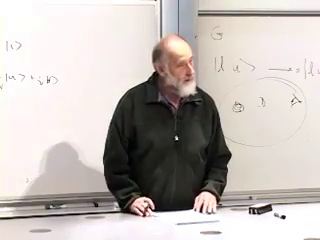
\includegraphics[width=0.66\textwidth]{lecture_07_figure_06.png}
\caption{지정된 켓에서 앙상블 기술로 넘어가는 개념적 전환.}
\lectureframe{01:29:43}
\end{figure}

상태 \(|i\rangle\)를 확률 \(\rho_i\)로 준비하면 밀도 연산자는 다음과 같습니다.
\begin{equation}
\rho=\sum_i\rho_i|i\rangle\langle i|.
\end{equation}
준비 기저에서는 다음과 같습니다.
\begin{equation}
\rho=
\begin{pmatrix}
\rho_1&0&0&\cdots\\
0&\rho_2&0&\cdots\\
0&0&\rho_3&\cdots\\
\vdots&\vdots&\vdots&\ddots
\end{pmatrix}.
\end{equation}

\begin{figure}[htbp]
\centering
\includegraphics[width=0.68\textwidth]{lecture_07_figure_09.png}
\caption{대각 밀도행렬과 그 정규화 조건.}
\lectureframe{01:32:12}
\end{figure}

고윳값은 실수이며 음이 아닌 값이고, 확률의 정규화 조건은 다음과 같습니다.
\begin{equation}
\operatorname{Tr}\rho=\sum_i\rho_i=1.
\end{equation}

\(F\)을 에르미트 관측가능량이라고 합시다. 앙상블의 기댓값은 다음과 같습니다.
\begin{equation}
\langle F\rangle=\operatorname{Tr}(F\rho).
\end{equation}

\begin{figure}[htbp]
\centering
\includegraphics[width=0.68\textwidth]{lecture_07_figure_10.png}
\caption{트레이스로 나타낸 기댓값 \(\langle F\rangle=\operatorname{Tr}(F\rho)\).}
\lectureframe{01:35:05}
\end{figure}

일반적인 가중평균을 얻으려면 \(\rho\)가 대각화된 기저에서 트레이스를 계산하고 항등 연산자의 분해를 대입하면 됩니다.
\begin{align}
\operatorname{Tr}(F\rho)
&=\sum_i\langle i|F\rho|i\rangle\\
&=\sum_{i,j}\langle i|F|j\rangle
               \langle j|\rho|i\rangle\\
&=\sum_i\rho_i\langle i|F|i\rangle.
\end{align}
따라서 각 순수 상태의 기댓값에는 그 상태가 준비되었을 확률이 가중치로 주어집니다.

트레이스에는 다음과 같은 순환 성질이 있습니다.
\begin{equation}
\operatorname{Tr}(AB)=\operatorname{Tr}(BA),
\end{equation}
\(A\)와 \(B\)가 서로 가환하지 않더라도 성립합니다. 따라서 \(\operatorname{Tr}(F\rho)=\operatorname{Tr}(\rho F)\)입니다.

\section{양자 엔트로피와 뒤로 미룬 결론}

밀도행렬의 엔트로피는 다음과 같습니다.
\begin{equation}
S(\rho)=-\operatorname{Tr}(\rho\log\rho).
\end{equation}
\(\log\rho\)와 같은 함수는 에르미트 양의 연산자의 고윳값을 통해 정의됩니다. 만약
\begin{equation}
\rho=\sum_i\rho_i|i\rangle\langle i|,
\end{equation}
라면,
\begin{equation}
\log\rho=\sum_{\rho_i>0}(\log\rho_i)|i\rangle\langle i|,
\end{equation}
따라서 다음과 같습니다.
\begin{equation}
S(\rho)=-\sum_i\rho_i\log\rho_i.
\end{equation}

\begin{figure}[htbp]
\centering
\includegraphics[width=0.68\textwidth]{lecture_07_figure_11.png}
\caption{고전 엔트로피 공식을 \(S=-\operatorname{Tr}(\rho\log\rho)\)로 다시 쓴 표현.}
\lectureframe{01:41:25}
\end{figure}

알려진 순수 상태의 밀도 연산자는 다음과 같습니다.
\begin{equation}
\rho_\psi=|\psi\rangle\langle\psi|,
\end{equation}
고윳값은 \(1,0,\ldots\)이므로 \(S(\rho_\psi)=0\)입니다. 이는 \(|\psi\rangle\)에 대한 모든 측정에서 결과가 확정되어 있다는 뜻은 아닙니다. 준비된 상태에 대해 추가적인 통계적 무지가 없다는 뜻입니다. 정반대의 경우는 다음과 같습니다.
\begin{equation}
\rho=\frac{I}{d}
\qquad\Longrightarrow\qquad
S(\rho)=\log d,
\end{equation}
여기서 \(d=\dim\mathcal H\)입니다. 최대 혼합 상태는 모든 직교 방향에 같은 가중치를 부여합니다.

얽힘과의 연관성은 이제 가까워졌지만, 아직 구체적으로 전개하지 않았습니다. 합성계 \(AB\)가 공동 상태에 있고 모든 실험이 \(A\)에만 한정된다고 하자. \(B\)를 무시한 채 \(A\)에서 얻을 수 있는 모든 기댓값을 재현하는 대상이 있어야 합니다. 그 대상이 \(A\)의 밀도행렬입니다. 공동 상태가 인수분해되면 \(A\)의 밀도행렬은 순수 상태이며 엔트로피는 영입니다. \(A\)와 \(B\)가 얽혀 있으면 \(A\)의 밀도행렬은 일반적으로 혼합 상태이며 엔트로피는 영이 아닙니다. 이 축약 밀도행렬을 구성하고 엔트로피를 계산하는 일은 다음 강의에서 다룰 내용입니다.
